\documentclass[12pt,a4paper,UTF8]{ctexart}
\CTEXsetup[format={\Large\bfseries}]{part}
\CTEXsetup[format={\Large\bfseries}]{section}

\usepackage{ctex}
\usepackage{xcolor}
\usepackage{listings}
\usepackage{commath}
\usepackage{gbt7714}
\usepackage{graphicx}
\usepackage{rotating}
\usepackage{hyperref}
\usepackage{booktabs}
\usepackage{amsfonts}
\usepackage{fancyhdr} %调用页眉页脚宏包

% 用来设置附录中代码的样式
\lstset{
    basicstyle          =   \sffamily,          % 基本代码风格
    keywordstyle        =   \bfseries,          % 关键字风格
    commentstyle        =   \rmfamily\itshape,  % 注释的风格,斜体
    stringstyle         =   \ttfamily,  % 字符串风格
    flexiblecolumns,                % 别问为什么,加上这个
    numbers             =   left,   % 行号的位置在左边
    showspaces          =   false,  % 是否显示空格,显示了有点乱,所以不现实了
    numberstyle         =   \zihao{-5}\ttfamily,    % 行号的样式,小五号,tt等宽字体
    showstringspaces    =   false,
    captionpos          =   t,      % 这段代码的名字所呈现的位置,t指的是top上面
    frame               =   lrtb,   % 显示边框
}

\lstdefinestyle{Python}{
    language        =   Python, % 语言选Python
    basicstyle      =   \zihao{-5}\ttfamily,
    numberstyle     =   \zihao{-5}\ttfamily,
    keywordstyle    =   \color{blue},
    keywordstyle    =   [2] \color{teal},
    stringstyle     =   \color{magenta},
    commentstyle    =   \color{red}\ttfamily,
    breaklines      =   true,   % 自动换行,建议不要写太长的行
    columns         =   fixed,  % 如果不加这一句,字间距就不固定,很丑,必须加
    basewidth       =   0.5em,
}

% \title{标 题}
% \author{heshiyu}
% \date{\today}


\begin{document}
% \maketitle
% \pagestyle{fancy}
% \fancyhf{} % 清除所有页眉页脚
% % \renewcommand{\headrulewidth}{0pt} % 去页眉线
% \fancyfoot[R]{\thepage} % 设置右页脚为页码
% \fancyhead[R]{\leftmark} % 设置右页眉为章节标题
\tableofcontents

\part{课程论文题目}
人工智能基本理论及应用研究综述

本文选取 \LaTeX 作为文章撰写工具。

本文参考文献格式为GB/T 7714-2015-numerical。
\part{课程论文内容}
\section{知识表示与推理}
\subsection{知识与知识表示}
\textrm{知识可以理解为事实和与事实相关的规则的集合。与之类似的是离散数学中的命题逻辑的概念,众所周知命题便是各种事实以及事实之间的推断。和命题逻辑一眼样,人工智能领域中的知识也是为了反应事物或者说是事实之间的联系与规则。相较与命题逻辑,此处的知识要求更高一些,我们希望知识至少是相对正确的(相对正确性),希望知识可以用符号等显式的表示出来以便能更好的利用这些知识(可表示、可利用性),当然知识也有很多不确定性。在不同的先决条件或者不同的规则下,所得到的知识也大相径庭。例如生物领域中“橘生淮南则为橘 生于淮北则为枳”,计算机科学中二进制10与十进制的10并不相同。}

\textrm{知识表示不仅在人工智能领域中出现,其还是认知科学领域的重要内容,在AI领域,我们通常希望将知识表示训练的像人一样智慧。}

\begin{enumerate}
    \item AI知识表示:
    \begin{description}
        \item [表示方法] 我们如何表示知识?
        \item [表示范围] 某一表示方法的使用范围?
        \item [表示效果] 某种表示方案的效果如何?
        \item [本身性质] 知识表示本身的性质问题?
    \end{description}
\end{enumerate}

知识表示分为两个步骤,将我们生活中的信息流转化为程序可以识别的信息流,然后模仿人的感知、认知、推理等思维来解决一些人类遇到的费时费力的艰巨任务。

对于AI领域的知识表示,通常有以下方法,见表~\ref{table:知识表示方法应用}。

对于AI中各种知识表示方法的优劣,见表~\ref{table:知识表示方法优劣}。

而另一块是关于确定性推理的概念,即依据我们现有的初始信息或依据,按某种确定的推理策略不断运用库中已有知识来逐步得到确定的结论的推理过程。
而在AI领域,我们的推理是借助程序也叫推理机实现的。
\begin{table}[htpb]
    \centering
    \caption{知识表示方法及应用.}
    \label{table:知识表示方法应用}
    \begin{tabular}{@{}cc@{}}
    \toprule
    知识表示方法               & 应用                                                              \\ \midrule
    一阶谓词逻辑表示法            & 知识表示与推理                                                         \\
    \multicolumn{1}{l}{} &                                                                 \\
    产生式表示法               & \begin{tabular}[c]{@{}c@{}}基于遗传算法的问题求解系统\\ 图搜索求解模型\end{tabular} \\
    \multicolumn{1}{l}{} &                                                                 \\
    框架表示法                & 复杂知识的框架网络                                                       \\
    \multicolumn{1}{l}{} &                                                                 \\
    语义网络表示法              & 机器翻译、问答系统、自然语言理解                                                \\ \bottomrule
    \end{tabular}
\end{table}
\begin{table}[htpb]
    \centering
    \caption{各种知识表示方法的优劣.}
    \label{table:知识表示方法优劣}
    \begin{tabular}{@{}ccc@{}}
    \toprule
    知识表示方法               & 优势                                                                           & 劣势                                                                              \\ \midrule
    一阶谓词逻辑表示法            & 自然精确严密易实现                                                                    & \begin{tabular}[c]{@{}c@{}}不能表示不确定的知识\\ 耦合度高,效率低\end{tabular}                   \\
    \multicolumn{1}{l}{} & \multicolumn{1}{l}{}                                                         & \multicolumn{1}{l}{}                                                            \\
    产生式表示法               & \begin{tabular}[c]{@{}c@{}}自然、模块性\\ 有效性、清晰性\end{tabular}                     & \begin{tabular}[c]{@{}c@{}}不能表达具有结构性的知识\\ 效率不高\end{tabular}                     \\
    \multicolumn{1}{l}{} & \multicolumn{1}{l}{}                                                         & \multicolumn{1}{l}{}                                                            \\
    框架表示法                & 结构性、继承性、自然性                                                                  & \begin{tabular}[c]{@{}c@{}}缺乏形式理论\\ 适应能力不强\end{tabular}                         \\
    \multicolumn{1}{l}{} & \multicolumn{1}{l}{}                                                         & \multicolumn{1}{l}{}                                                            \\
    语义网络表示法              & \begin{tabular}[c]{@{}c@{}}强调联系,符合人类思维\\ 描述明确简洁直观\\ 结构化显性描述语义关系\end{tabular} & \begin{tabular}[c]{@{}c@{}}不能保证推论的严格有效\\ 不能处理结点太多的推理\\ 不便表达判断性深层知识\end{tabular} \\ \bottomrule
    \end{tabular}
\end{table}

\subsection{确定性推理}
常见的确定性推理方法有图搜索策略,盲目搜索和启发式搜索等,还有最新的像消解原理
、规则演绎系统以及产生式系统。确定性推理的特点见表~\ref{table:qdx特点},此处我选择启发式搜索(Heuristic)来介绍他的原理和应用。
\begin{table}[htb]
    \centering
    \caption{确定性推理特点.}
    \label{table:qdx特点}
    \begin{tabular}{@{}cc@{}}
    \toprule
    确定的推理策略、确定的结论                             \\ \hline
    \multicolumn{1}{l}{事实(条件)和知识是构成推理的两个基本要素} \\ \hline
    以数理逻辑的有关理论、方法和技术为理论基础                     \\ \hline
    机械化的、可在计算机上加以实现                           \\ \hline
    \toprule
    \end{tabular}
\end{table}
\subsubsection{确定性推理方法之启发性搜索算法}
启发式搜索方法是一种帮你不断试探出答案的方法,但它给出的答案是具有偶然性的,也就是subject to chance。
如在一个状态空间中,对一点的可能所在的每一个位置进行评估,先得到一个最可能的位置。
再从这个位置出发持续进行下一轮的位置评估,这样的循环往复的搜索过程就被称为启发式搜索。
而评估过程所用到的估价函数是启发式搜索核心,可以根据状态场景来选取合适的估价函数,
常见的如式~\ref{eq:启发式搜索估价}:
\begin{equation}
    f(n)=g(n)+h(n)
    \label{eq:启发式搜索估价}
\end{equation}
\subsubsection{一种启发性搜索算法的应用}
天气被认为是影响航班路径规划的最主要因素,有70\%的航班延误是由于危险天气\cite{Narkawicz2016}。
Li He和Anfei Zhao\cite{hePathPlanningMethod2019}使用启发式算法将飞机在危险天气下,不同飞行海拔高度对飞机飞行转态的影响离散化进入一个多边网格模型,
结果发现,借助该网格所获得的最小代价的飞行路径比传统的以一个恒定海拔高度飞行的飞行路径要更短。
本章认为,当飞行过程中海拔发生变化,则规划的飞行路径也应适当的变化,详情见图~\ref{fig:path plan change }。
\begin{figure}[htbp]
    \centering
    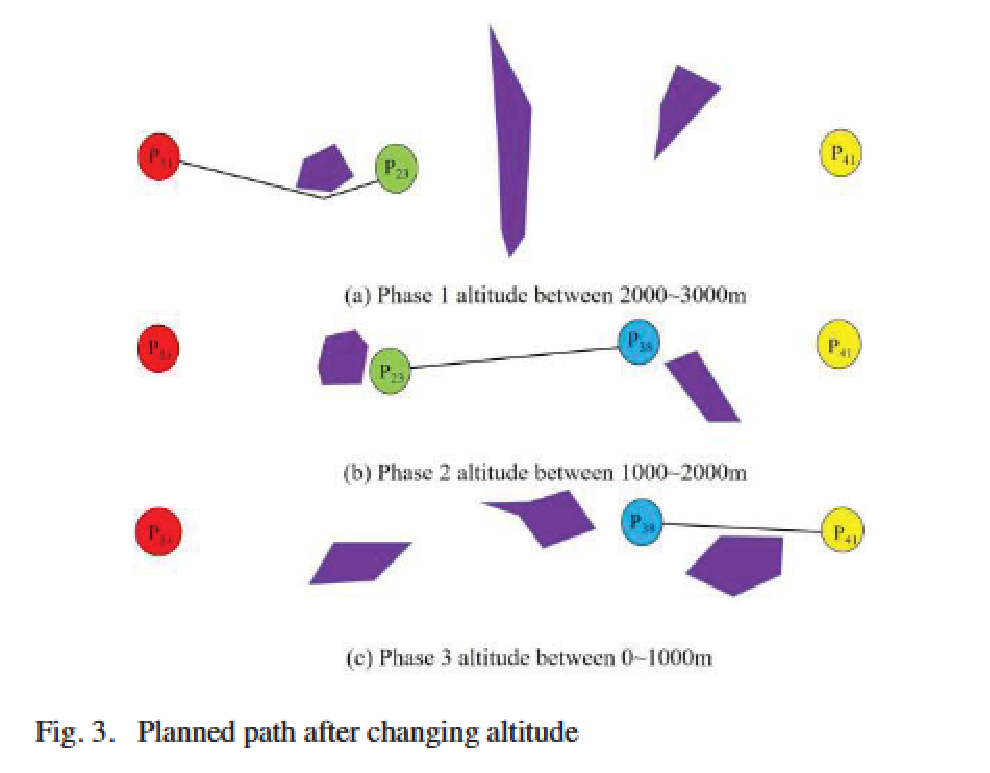
\includegraphics[width=12cm]{allpicture/altitude_change.eps}
    \caption{海拔变化时路径节点变化图.}
    \label{fig:path plan change }
\end{figure}

这篇文章讨论,如果在决策点改变飞行高度,则从决策点到达下一个路径点的成本不是水平面上的欧几里德距离。
因为高度变化被视为在一定爬升角度下的直线飞行,计算到达所选高度后的下一个路径点的代价公式为式~\ref{eq:代价C_height}
\begin{equation}
    C_{\text {height }}=\sqrt{d^2{ }_{\text {height }}+h^2}
    \label{eq:代价C_height}
\end{equation}

$ d_{\text {height }} $是当前决策点与选定高度中的下一个路径点在水平面上的欧几里得距离,$ h $是海拔的变化。
同时,在网格系统中,使用曼哈顿距离作为代价估计的启发式函数具有更好的计算速度和搜索效率\cite{grecheComparisonEuclideanManhattan2017}。
这样做可以确保路径搜索方向始终靠近目标,简化搜索空间,排除远离目标的点。得到的启发式搜索函数中$ h(n) $为~式~\ref{eq:h(n)}。
\begin{equation}
    h(n)=\left|x_g-x_n\right|+\left|y_g-y_n\right|
    \label{eq:h(n)}
\end{equation}
$ n $表示当前网格点,$ g $表示目标点,$ x_g, x_n$等表示相应结点坐标。

则应用次启发式搜索的规划飞行路径的代价函数就为式~\ref{eq:启发式搜索cost函数},$ C_{\text {height }} $表示到达当前结点n之前的代价。
\begin{equation}
    f(n)=C_{\text {height }}+\left|x_g-x_n\right|+\left|y_g-y_n\right|
    \label{eq:启发式搜索cost函数}
\end{equation}

最终的实验结果表明,根据危险天气和海拔的不同,基于启发式搜索的路径决策算法所得到的航班里程要小于恒定海拔下飞行的航班里程。
通过海拔的不断调整,可以将飞机更好的锁定在危险天气影响较小的飞行区域,进而减少平均航行里程\cite{hePathPlanningMethod2019}。

\subsection{不确定性推理}
对比于上文中所讲的确定性推理,不确定性推理便好理解了。
不确定性推理的初始的条件(论据)不确定,推理方法(或策略)也不确定,知识库也不确定,最后的推理结果不确定但合理。
常见的知识不完备、不精确以及模糊知识等的推理也属于不确定推理的范畴。不确定性推理的特点见表~\ref{table:bqdx特点}
\begin{table}[htb]
    \centering
    \caption{不确定性推理特点.}
    \label{table:bqdx特点}
    \begin{tabular}{@{}cc@{}}
    \toprule
    证据的不确定性表示                       \\ \hline
    不确定性的匹配                         \\ \hline
    \multicolumn{1}{l}{组合证据不确定性的计算} \\ \hline
    不确定性的更新                         \\ \hline
    不确定性结论的合成                       \\ \hline
    \toprule
    \end{tabular}
\end{table}
\subsubsection{不确定性推理之主观贝叶斯方法}
常见的不确定性推理方法有模糊推理、可信度、证据理论、主观贝叶斯方法等等。本文主要选取主观贝叶斯
方法来着重介绍一下。主观贝叶斯方法隶属于规则推理方法,其以贝叶斯理论为依据,克服了实际问题中很难获取到先验概率的问题。\cite{gonenComparingObjectiveSubjective2019}\cite{uzunogluAdaptiveBayesianApproach2020a}
我们都知道贝叶斯公式为式~\ref{eq:bayes},而将全概率公式代入后可得贝叶斯公式的另一种形式,即式~\ref{eq:全概率Bayes}。
\begin{equation}
    P\left(A_i \mid B\right)=\frac{P\left(A_i\right) \times P\left(B \mid A_i\right)}{P(B)}, i=1,2, \ldots, n
    \label{eq:bayes}
\end{equation}

\begin{equation}
    \label{eq:全概率Bayes}
    P\left(A_i \mid B\right)=\frac{P\left(A_i\right) \times P\left(B \mid A_i\right)}{\sum_{j=1}^n P\left(A_j\right) \times P\left(B \mid A_j\right)}
    \end{equation}

引入产生式规则IF E THEN Hi,用该规则的前提条件E代替Bayes公式中的B,而$ A_i $则由$ H_i $来代替可得到公式~\ref{eq:HI|E公式}。
\begin{equation}
    \label{eq:HI|E公式}
    P\left(H_i \mid E\right)=\frac{P\left(E \mid H_i\right) P\left(H_i\right)}{\sum_{j=1}^n P\left(E \mid H_j\right) P\left(H_j\right)}, i=1,2, \ldots, n
\end{equation}
再引入一组不确定性数值对$ (\mathrm{LS}, \mathrm{LN}) $来表示知识的强度,分别称为充分性度量和必要性度量,即式~\ref{eq:LS}和式~\ref{eq:LN}。
\begin{equation}
    \label{eq:LS}
    L S=\frac{P(E \mid H)}{P(E \mid \neg H)}
\end{equation}
\begin{equation}
    \label{eq:LN}
    L N=\frac{P(\neg E \mid H)}{P(\neg E \mid \neg H)}=\frac{1-P(E \mid H)}{1-P(E \mid-\neg H)}
\end{equation}
则此时得到主观贝叶斯公式为式~\ref{eq:主观Bayes}。
\begin{equation}
    \label{eq:主观Bayes}
    \begin{gathered}
    P(H \mid E)=\frac{P(H) \times P(E \mid H)}{P(E)} \\
    P(\neg H \mid E)=\frac{P(\neg H) \times P(E \mid \neg H)}{P(E)}
    \end{gathered}
\end{equation}
借助几率函数即式~\ref{eq:几率函数}最终可得到分段线插值表示的后验概率为式~\ref{eq:分段Bayes}。
\begin{equation}
    \label{eq:几率函数}
    \begin{gathered}
    O(x)=\frac{P(x)}{1-P(x)}=\frac{P(x)}{P(-x)} \\
    P(x)=\frac{O(x)}{1+O(x)} \\
    P(x)=0 \text { 时, } O(x)=0 \\
    P(x)=1 \text { 时, } O(x)=+\infty
    \end{gathered}
\end{equation}
\begin{equation}
    \label{eq:分段Bayes}
    P(H \mid S)=\left\{\begin{array}{c}
    P(H \mid \neg E)+\frac{P(H)-P(H \mid \neg E)}{P(E)} \times P(E \mid S), 0 \leq P(E \mid S)<P(E) \\
    P(H)+\frac{P(H \mid E)-P(H)}{1-P(E)} \times[P(E \mid S)-P(E)], P(E) \leq P(E \mid S) \leq 1 \\
    \end{array}\right.
\end{equation}
其中S是对E的观察,而P(E|S)表示在观察S下,E发生的概率。
\subsubsection{一种主观贝叶斯方法的应用}
袁杰等\cite{YuanJiYuGaiJinZhuGuanBeiYeSiFangFaShiBieDianRongMeiLuYiChangGongKuang2021}借助改进后的主观贝叶斯方法来
更好的进行电熔镁炉熔炼过程异常工况识别,同时利用模糊隶属度函数对个观测状态和证据进行匹配,对金属熔炼过程中的不确定性问题即异常工况
获取到更好的识别效果。

这篇文章考虑到主观贝叶斯公式里$ L_S $和$ L_N $的取值较大,而选择将其值限制在[0, 1]中,并设置$ P_x $为证据A发生时对结论B的支持度。
并选择合适的映射函数$ f $,即e指数函数式~\ref{func:e映射函数}。
\begin{equation}
    \label{func:e映射函数}
    1-k_1 \mathrm{e}^{-k_2 L_{\mathrm{S}}}=p_x
\end{equation}
从而得到新的$ L_S $和$ L_N $的概率公式~\ref{eq:LS_new}和~\ref{eq:LN_new}。
\begin{equation}
    \label{eq:LS_new}
    L_{\mathrm{S}}=\frac{\ln \left(1-p_x\right)}{\ln (1-P(B))}
\end{equation}
\begin{equation}
    \label{eq:LN_new}
    L_{\mathrm{N}}=\frac{\ln \left(1-p_y\right)}{\ln (1-P(B))}
\end{equation}
并借助命题事件$ x \geq x_{\mathrm{a}} $模糊隶属度函数图~\ref{fig:模糊隶属度函数}来获得某证据A在观察S情况下匹配程度$ P(A \mid S) $,
即特征变量观测值S特征变量限定范围A的匹配关系。
改进了传统的主观贝叶斯方法中证据与结论的匹配非0即1(即只有匹配或不匹配的结果)。
也提高了异常工况识别中的识别准确率。
\begin{figure}[htbp]
    \centering
    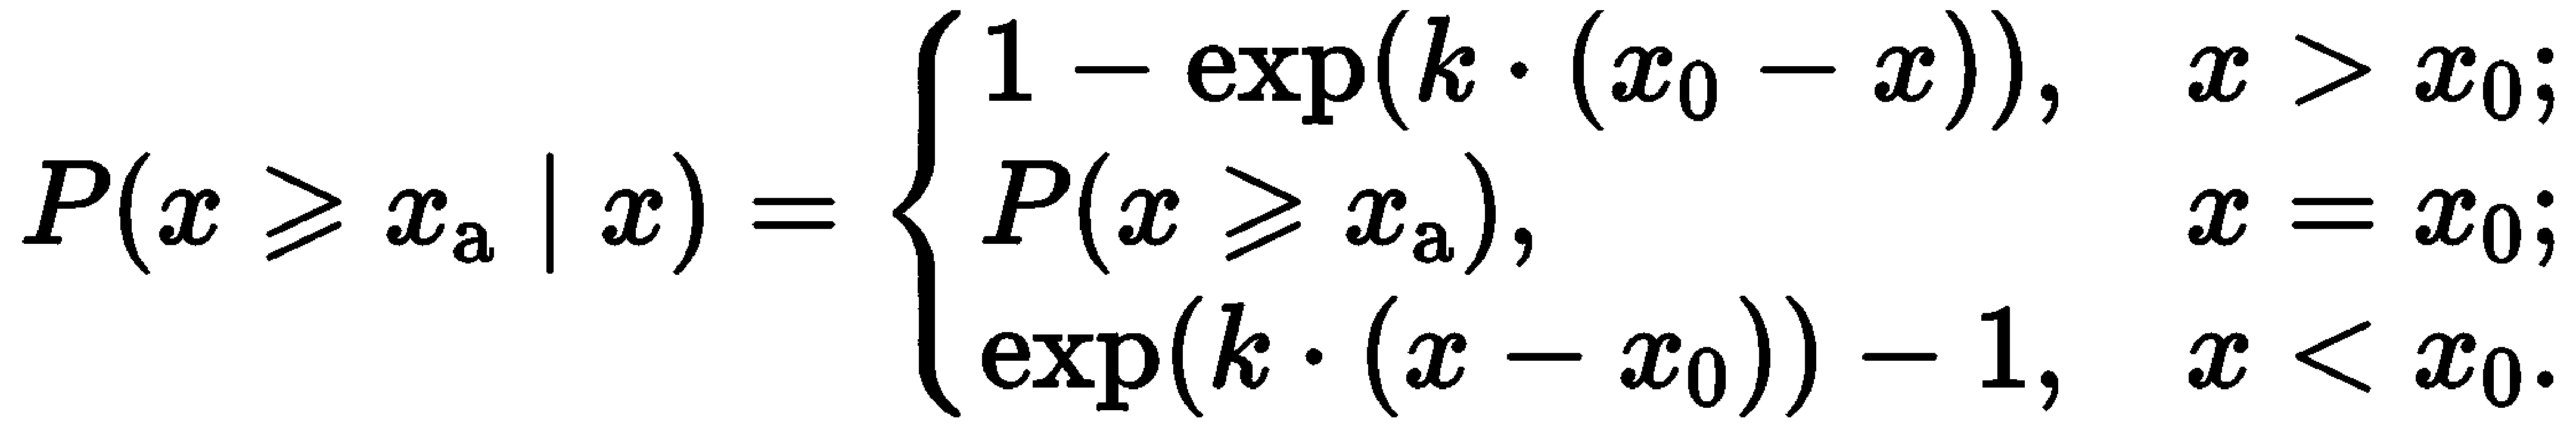
\includegraphics[width=12cm]{allpicture/a8ls3-uktor.eps}
    \caption{命题模糊隶属度函数.}
    \label{fig:模糊隶属度函数}
\end{figure}

从现场收集并选取了200个异常工况样本,来制图显示电熔镁炉异常运行数据图,见图~\ref{fig:贝叶斯方法结果}。
\begin{figure}[htbp]
    \centering
    \includegraphics[width=12cm]{allpicture/ajop2-9xa4r.eps}
    \caption{两种贝叶斯方法异常工况识别结果.}
    {(a) —改进主观贝叶斯方法; (b) —传统主观贝叶斯方法}
    \label{fig:贝叶斯方法结果}
\end{figure}
可以看到,使用改进的主观贝叶斯方法对电熔镁炉熔炼工况进行识别后,相较于传统的主观贝叶斯方法,误识别
样本减少了40\%,说个改进的主观贝叶斯方法能对异常工况识别更快且提高诊断准确率\cite{YuanJiYuGaiJinZhuGuanBeiYeSiFangFaShiBieDianRongMeiLuYiChangGongKuang2021}。

可以发现主观贝叶斯方法的优点是理论基础比较坚实(计算公式多是由概率论的基础所推导出来),且
$ L_S $和$ L_N $由领域内的专家给出,避免了我们自己的数据统计工作。
再加上很多时候LS和LN也反映了证据与结论间的因果关系,也使得结论更为可靠。缺点是应用时,相关领域专家需要
同时给出先验概率P(H),又由于Bayes的独立性假设等等都很难满足,使得该方法使用受限。这也间接看出
该方法主要应用在领域专家能给出$ L_S $和$ L_N $以及事件满足独立性假设的情况,常见的如气象预测、人口预测等。

\section{搜索与问题求解}
\subsection{搜索与问题求解}
无信息搜索指的是已知条件很少,只有自己定义的信息可用,所以也称盲目式搜索。而有信息搜索就是找到一种策略来
判断某一种搜索到的状态比另一种更好,进而能朝向更优的方向不断搜索。而超越经典搜索(局部搜索)则不太关心搜搜过程中的
路径和代价,只关注解的状态。与之前的无信息搜索是在可观察、确定性以及已知的环境之下搜索不同,局部搜索跳出这些约束,不关心路径,从单个结点出发,
通常只移动到该结点的邻近状态,如果存在一个最优解,最优局部搜索状态通常能找到最优解对应的最大或者最小值。
\subsection{遗传算法及其改进方法在八皇后问题中的对比分析}
\subsubsection{遗传算法简介}
遗传算法是借鉴了达尔文生物进化学说中种群遗传、基因突变、自然选择和杂交等理论的一种进化搜索算法。
\begin{enumerate}
    \item 遗传算法的具体实现步骤:
    \begin{description}
        \item 生成随机候选群、初始化群基因个数。
        \item 设计适应度函数计算fitness\_value。
        \item 定义突变函数和交叉函数。
        \item 定义进化策略,包括丢弃和增补函数。
        \item 不断生成新种群,知道达到适应度要求的值。
    \end{description}
\end{enumerate}
\begin{figure}[htbp]
    \centering
    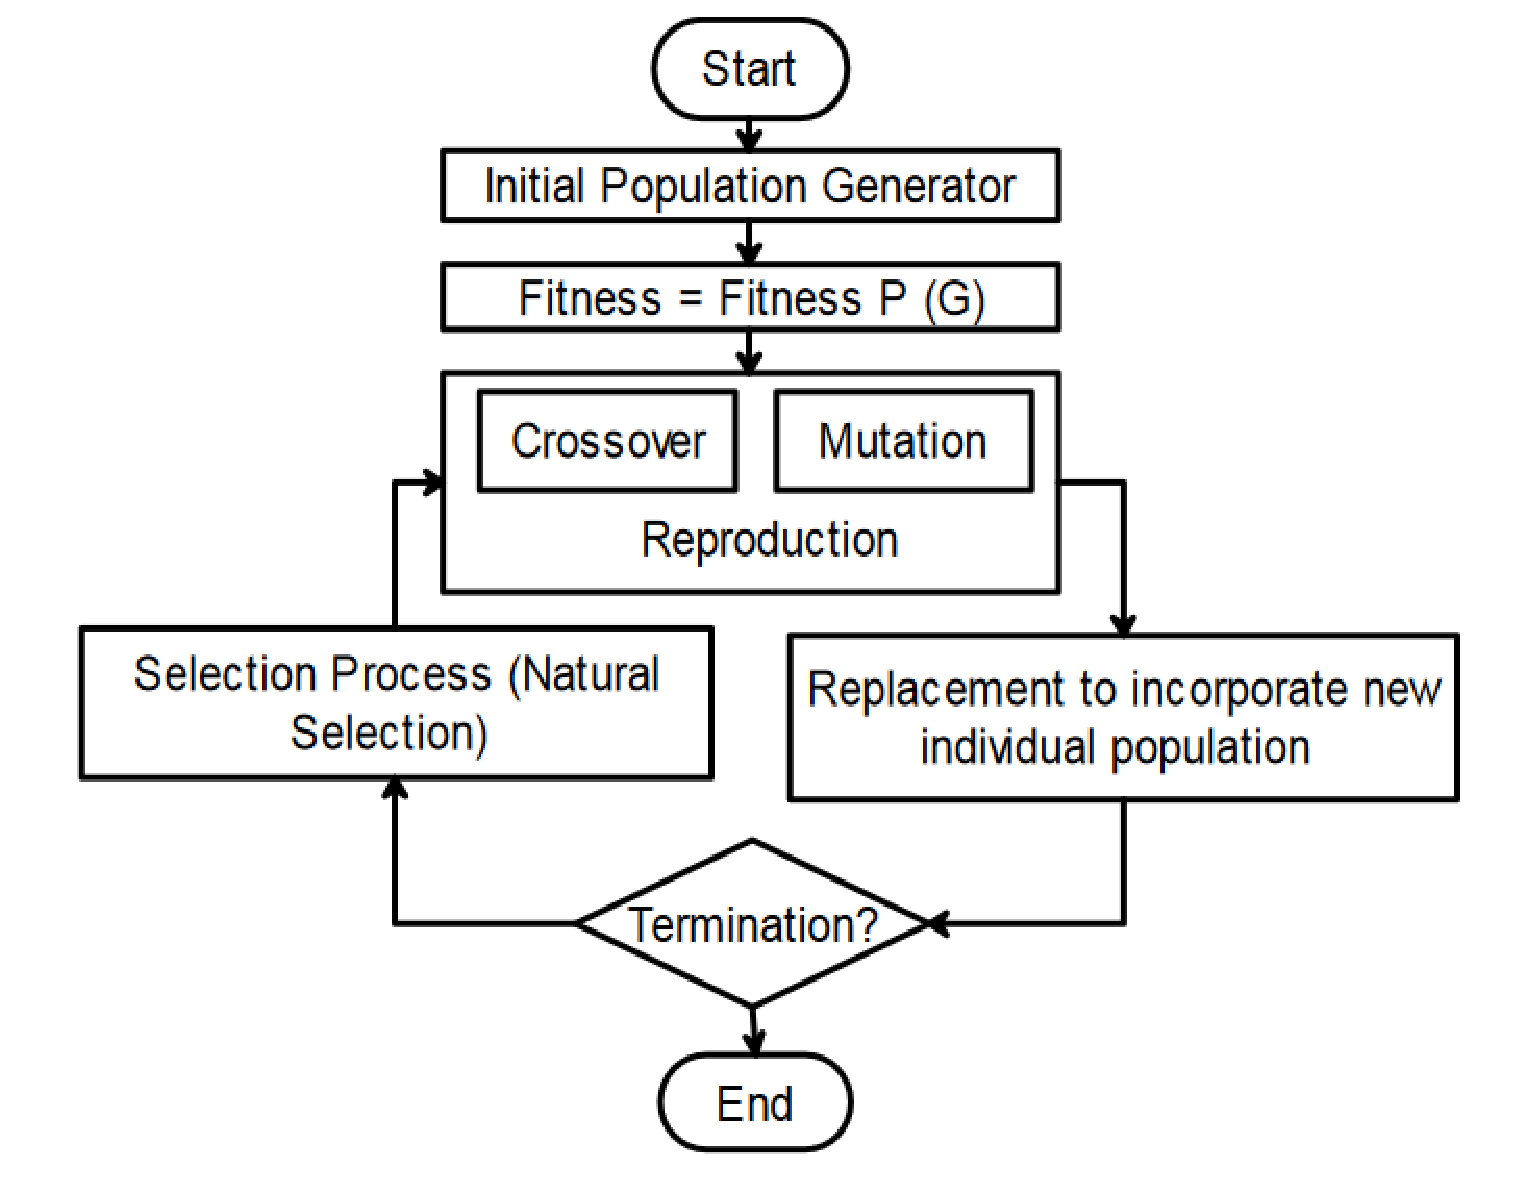
\includegraphics[width=12cm]{allpicture/alsxf-vpg1i.eps}
    \caption{简单遗传算法的步骤\cite{pandeyGeneticAlgorithmsConcepts2012}.}
    \label{fig:遗传算法的步骤}
\end{figure}
\subsubsection{遗传算法用于八皇后问题的介绍}
我们这次要解决的问题是八皇后问题,用八位数字来代表每个皇后,八个皇后组成遗传种群,并设置遗传种群的大小为100。
用不相互攻击的皇后对的数目来代表fitness\_value(即适应度值)。而如果检查次数(检查当前皇后位置是否与其他所有行列的皇后冲突)达到28,
则代表已找到八皇后的解。而是否选择该种群的某些个体进行下一轮的遗传则取决于个体的适应度值,适应度值越大,被选中的概率越高。
简单遗传算法的Python实现见列表\ref{Genetic_Algorithm_N_Queen.py},语言环境Python 3.8.13 64-bit。
\lstinputlisting[
    style       =   Python,
    caption     =   {简单遗传算法的Python实现\cite{EightQueensPuzzle}.},
    label       =   {Genetic_Algorithm_N_Queen.py}
]{Genetic_Algorithm_N_Queen.py}

\subsubsection{普通遗传算法解决八皇后问题的具体实现} 
根据种群中每个个体的fitness\_value在当前种群中总fitness\_value中的占比(即计算每个个体适应度值的概率分布)来选择一批用于繁衍下一代种群的新个体。
实验软件为Visual Studio Code. Version 1.56.2 测试平台:jupyter notebook,语言环境Python 3.8.13 64-bit。
采用这种策略的实验过程和结果见列表\ref{Normal_GeneticAlgorithm},图~\ref{fig:简单遗传算法的解8-Queen图}和图~\ref{fig:简单遗传算法的解收敛过程}。
\lstinputlisting[
    style       =   Python,
    caption     =   {简单遗传算法解决八皇后问题的测试过程和结果.},
    label       =   {Normal_GeneticAlgorithm}
]{Normal_GeneticAlgorithm.py}
\begin{figure}[htbp]
    \centering
    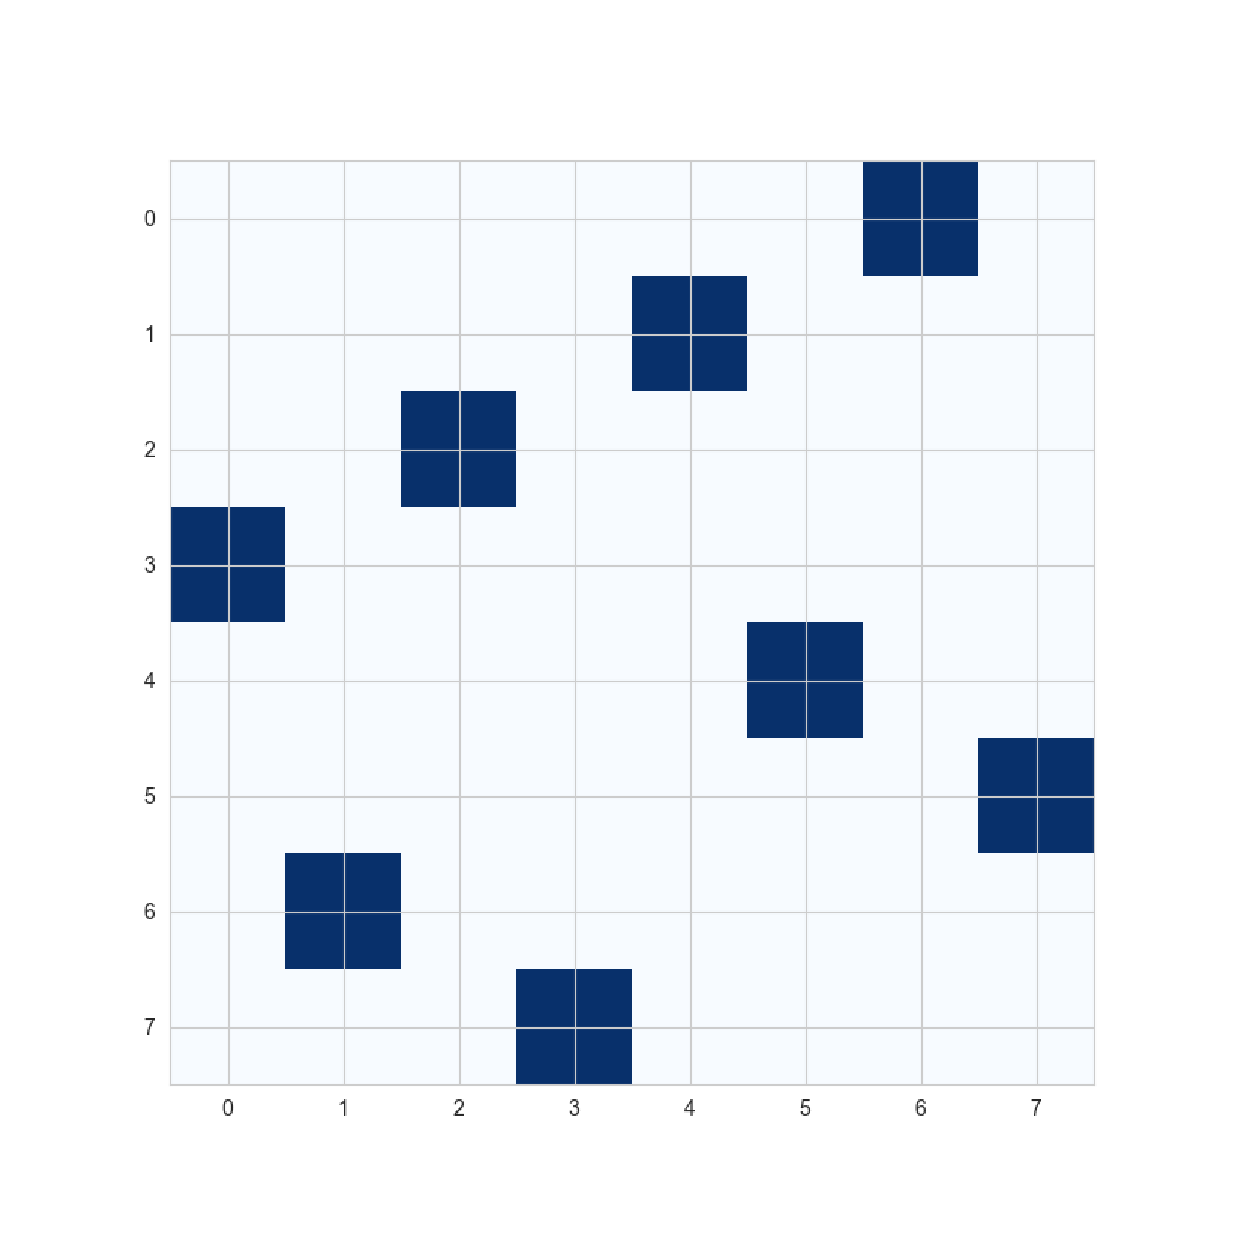
\includegraphics[width=6cm]{allpicture/queen100normal.eps}
    \caption{简单遗传算法的解8-Queen图.}
    \label{fig:简单遗传算法的解8-Queen图}
\end{figure}
\begin{figure}[htbp]
    \centering
    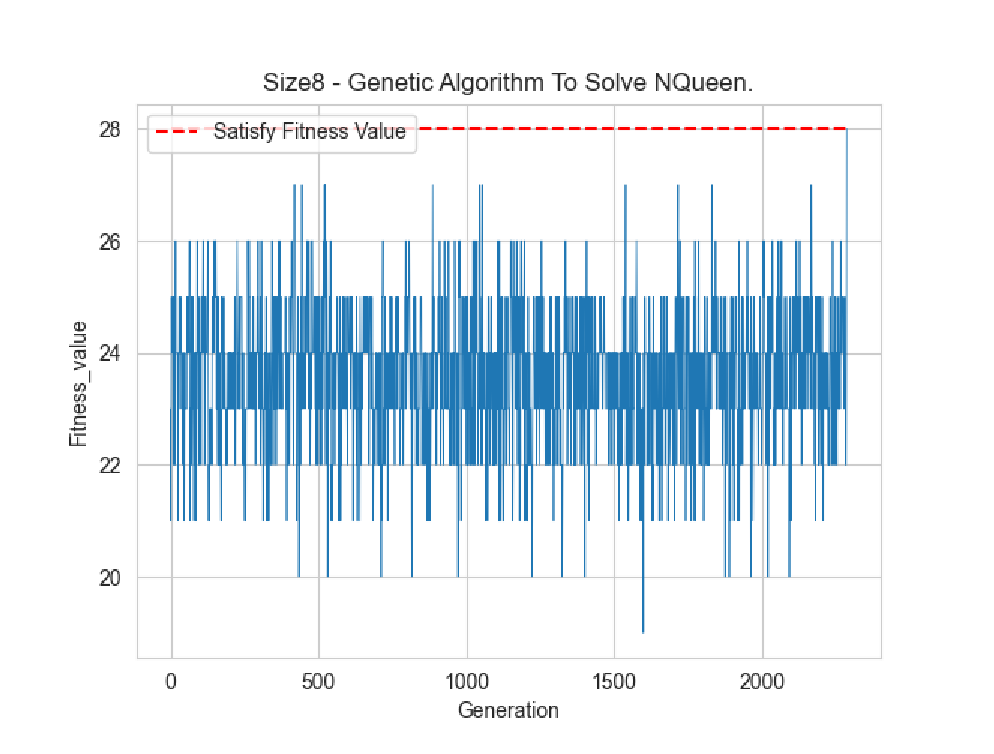
\includegraphics[width=8cm]{allpicture/generic100normal.eps}
    \caption{简单遗传算法的解收敛过程.}
    \label{fig:简单遗传算法的解收敛过程}
\end{figure}

\section{机器学习基本理论与方法}
\subsection{机器学习的基本概念及其学习策略}
机器学习也叫统计学习(Statistics Learning),就是利用现有数据或者知识并去寻找一些适合他的模型对其进行描述和表示
,并利用合适的模型对事物的发展和变化做一些合理的预测和分析,从而优化事务处理流程,提高决策的效率。
\begin{enumerate}
    \item 机器学习的三要素是:
    \begin{description}
        \item[模型(Model)] 模型就是数据里抽象出来的,那些刚好可以被拿来描述客观世界的数学特征或统计学框架。
        \item[策略(Strategy)] 通常在模型行为阶段用来评价模型的好坏,也可以称做是模型的比较标准和选择标准。
        \item[算法(Algorithm)] 有了数据和模型以及策略,就会在实际执行的过程中注重效率问题,这时候就需要优化模型和策略了,算法就是用来解决效率问题的优化方法。
    \end{description}
    \item 统计学习基本学习策略:
    \begin{description}
        \item 获取一个有限合理的训练数据集;
        \item 确定学习模型的集合(包含所有可能模型的假设空间);
        \item 确定学习策略(即选择准则);
        \item 实现学习算法;
        \item 通过学习方法选择最优模型;
        \item 利用学习到的最优化框架对新数据进行分析和预测。
    \end{description}
\end{enumerate}
\subsection{人工神经网络及其应用}
\subsubsection{人工神经网络的结构设计}
人工神经网络由input(输入),nerve cell(人工神经元),weights(权值),transfer function(传递函数),
activation function(激活函数),以及threshold(阈值)。一个人工神经系统的结构见图~\ref{fig:人工神经系统的结构}。
\begin{figure}[htbp]
    \centering
    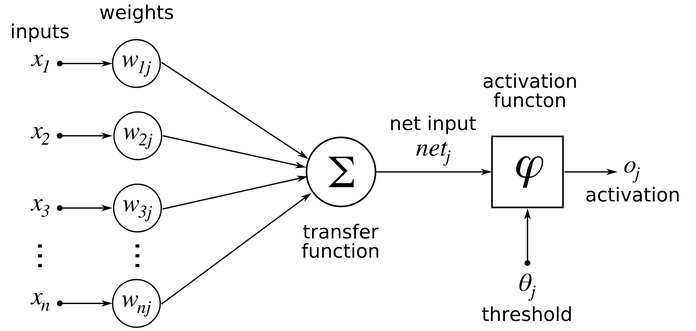
\includegraphics[width=12cm]{allpicture/v2-8b848443200436ac60334082e1f1e472_r.png}
    \caption{人工神经系统的结构.}
    \label{fig:人工神经系统的结构}
\end{figure}
其中核心是神经元,每个神经元input = sum(其他神经元的input x weight),并借助激活函数进行处理后将结果再传递给后面的
神经元,直到输出。这虽然看起来像是一系列简单的数学运算,但是如果将有限多层神经元堆叠起来,你就会获得一个能处理复杂任务的人工神经网络。
比如语音识别、图像识别分类等问题。

卷积神经网络、循环神经网络、玻尔兹曼机是三个常见的神经网络,下面我们用表格的形式来介绍
他们各自的特点和应用领域,见表~\ref{卷积神经网络和循环神经网络}。
\begin{table}[htbp]
    \centering
    \caption{卷积神经网络和循环神经网络的特点}
    \label{卷积神经网络和循环神经网络}
    \begin{tabular}{@{}cc@{}}
        \toprule
        名称   & 卷积神经网络                                                                                                        \\ \midrule
        特点   & \begin{tabular}[c]{@{}c@{}}核心层是Convolution + Pooling + FullConnected\\ 同时实现特征提取和分类\\ 能根据局部获得全局信息\end{tabular} \\
        应用领域 & 图像分类,目标检测跟踪,语义分割等                                                                                             \\ \midrule
        名称   & 循环神经网络                                                                                                        \\ \midrule
        特点   & \begin{tabular}[c]{@{}c@{}}可以根据借助时间序列的变化建模\\ 能有效处理序列特性的数据\end{tabular}                                        \\
        应用领域 & 视频分析、机器翻译、语音识别等                                                                                               \\ \bottomrule
    \end{tabular}
\end{table}
玻尔兹曼机是一种无监督深度学习模型,也是随机神经网络的一种。
玻尔兹曼机也是一种特殊形式的对数线性的马尔科夫随机场(Markov Random Field,MRF),即能量函数是自由变量的线性函数。
通过引入隐含单元,我们可以提升模型的表达能力,表示非常复杂的概率分布\cite{RenGongShenJingWangLuoArtificialNeurala}。他的特点如下:
\begin{enumerate}
    \item 玻尔兹曼机的特点:
    \begin{description}
        \item [学习阶段] 其权值设置或改变的算法是不确定的,通过某种概率分布不断变化调整。即每训练一次就可能改变一次。
        \item [运行阶段] 状态的改变也不是按照非0即1这样的确定性方式,同样按照某种概率分布(状态改变取1或0的概率)来进行状态的转移。
    \end{description}
\end{enumerate}
玻尔兹曼机中的受限玻尔兹曼机应用较多,主要应用是权重的初始化(让权重更有效的模拟数据)以及模型降维、分类和协同过滤,特征学习与主题建模等。
\subsubsection{人工神经网络的学习算法}
用于人工神经网络的学习算法有很多,Deeplearning Algorithms Tutorial(深度学习算法教程)一书将所有的人工智能算法应用总结如下\cite{DeeplearningAlgorithmsTutorial}:
\begin{itemize}
    \item 自动编码器(Autoencoder)
    \item 反向传播(Backpropagation)
    \item 递归神经网络(Recurrent Neural Network)
    \item 多层感知器(Multilayer Perceptron)
    \item 玻尔兹曼机(Boltzmann Machine)
    \item 卷积神经网络(Convolutional Neural Network)
    \item Hopfield网络(Hopfield Network)
    \item 径向基函数网络(Radial Basis Function Network)
    \item 受限玻尔兹曼机(Restricted Boltzmann Machine)
    \item 自组织映射(Self-Organizing Map)
    \item 尖峰神经网络(Spiking Neural Network)
\end{itemize}    
本文挑选比较常用的自动编码器算法、反向传播算法和受限玻尔兹曼机,并借助这些算法的相关应用文献来简要介绍。
\subsubsection{人工神经网络在与预测和图像方面的应用}
自动编码器(下文统称Autoencoder)其实是一种无监督的学习算法,用途主要在数据的降维和特征提取。
Autoencoder可以很好的学习input中的元素特征,且通过Autoencoder编码的数据在完成解码的同时较好的保留了原始数据信息。
Jiatong Shen等\cite{shenCreditCardFraud2021}使用一种基于深度神经网络的Autoencoder建立了一个信用卡欺诈预警系统,相比于传统的预警系统,该混合
系统的AUC(Area Under the Curve)值提高到了0.9577,被证明具有更好的准确性且稳定性更佳。

反向传播算法也称“误差反向传播”,可以计算网络中每个权重的损失函数梯度,,并反馈最优化方法用以不断更新权值的最小化损失函数。
S. Prashant Mahasagara和Andry Alamsyah等\cite{mahasagaraIndonesiaInfrastructureConsumer2017}
基于印度尼西亚基建和消费股股票价格历史走势,并借助人工神经网络的反向传播算法生成了一套相关行业股票价格的预测系统且可以以更小的误差率生成股票投资组合。
实验结果证明,在当前市场投资风险较低、股票市场波动较小时,使用ANN反向传播的预测系统要优于实际的真实投资。

上一个小章节我们介绍过玻尔兹曼机,这次我们要介绍的受限玻尔兹曼机是玻尔兹曼机的一种特殊拓扑结构,实质是一种概率图模型。
受限是指限定模型为二分图,模型包含两部分,即可见单元和隐单元,对应输入参数和训练结果。为了比一般的玻尔兹曼机的训练算法更高效,
二分图各边均连接可见单元与隐单元。
\begin{figure}[htpb]
     \centering
     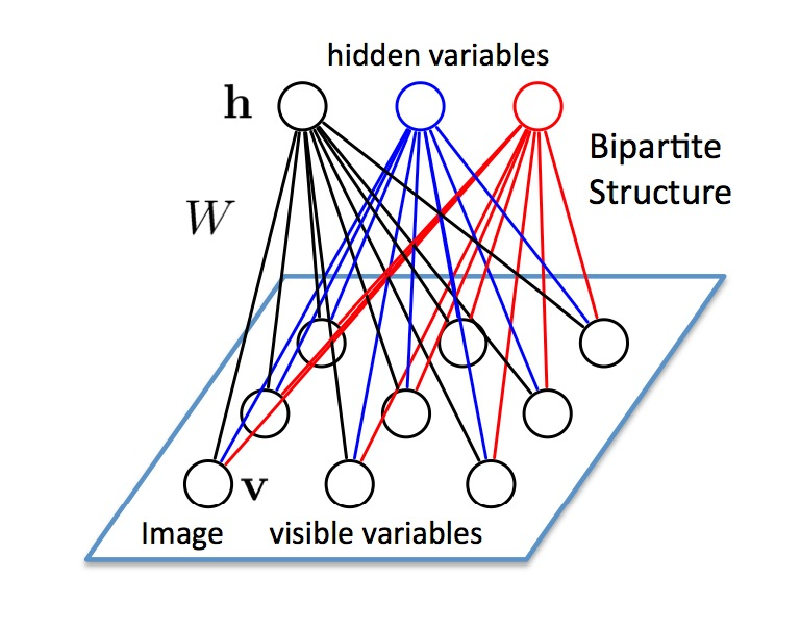
\includegraphics[width=0.6\textwidth]{allpicture/f5dt7-uxdal.eps}
     \caption{受限玻尔兹曼机}
     \label{fig:受限玻尔兹曼机}
\end{figure}
众所周知受限玻尔兹曼机(下统称RBM)的计算密度或强度较大,目前也有很多更快的训练算法被发展,
如GPU/CPU加速算法、硬件改进以及神经元友好型加速算法,这使得大型RBMs在未来的应用变得可能。

图像领域传统的字典学习算法收敛速度缓慢、训练稀疏表示的如图~\ref{fig:图像稀疏表示图}效果学习效果差、如果被噪声干扰学习效果会更糟糕。
\begin{figure}[htpb]
    \centering
    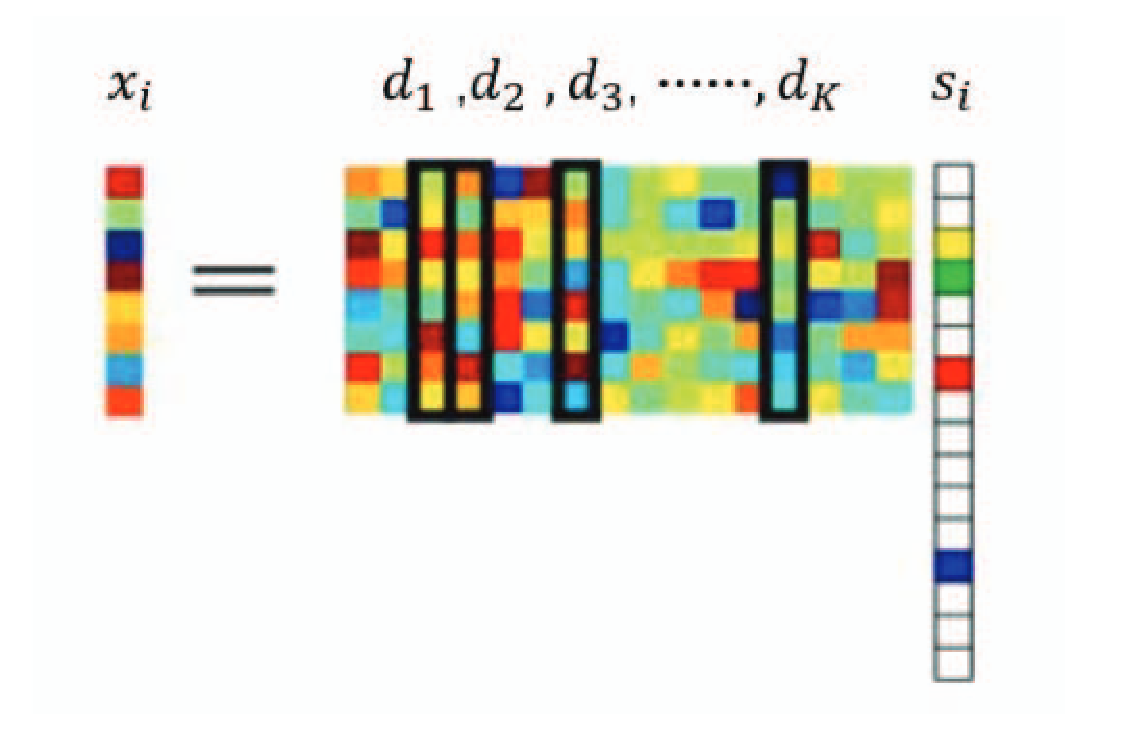
\includegraphics[width=0.8\textwidth]{allpicture/图像稀疏表示图.eps}
    \caption{图像稀疏表示图}
    \label{fig:图像稀疏表示图}
\end{figure}
为了解决这个问题,Liu Lian等\cite{lianDictionaryLearningAlgorithm2021}提出了一种基于受限玻耳兹曼机的字典学习算法。
字典学习的神经网络结构见图~\ref{fig:字典学习神经网络结构}
\begin{figure}[htpb]
    \centering
    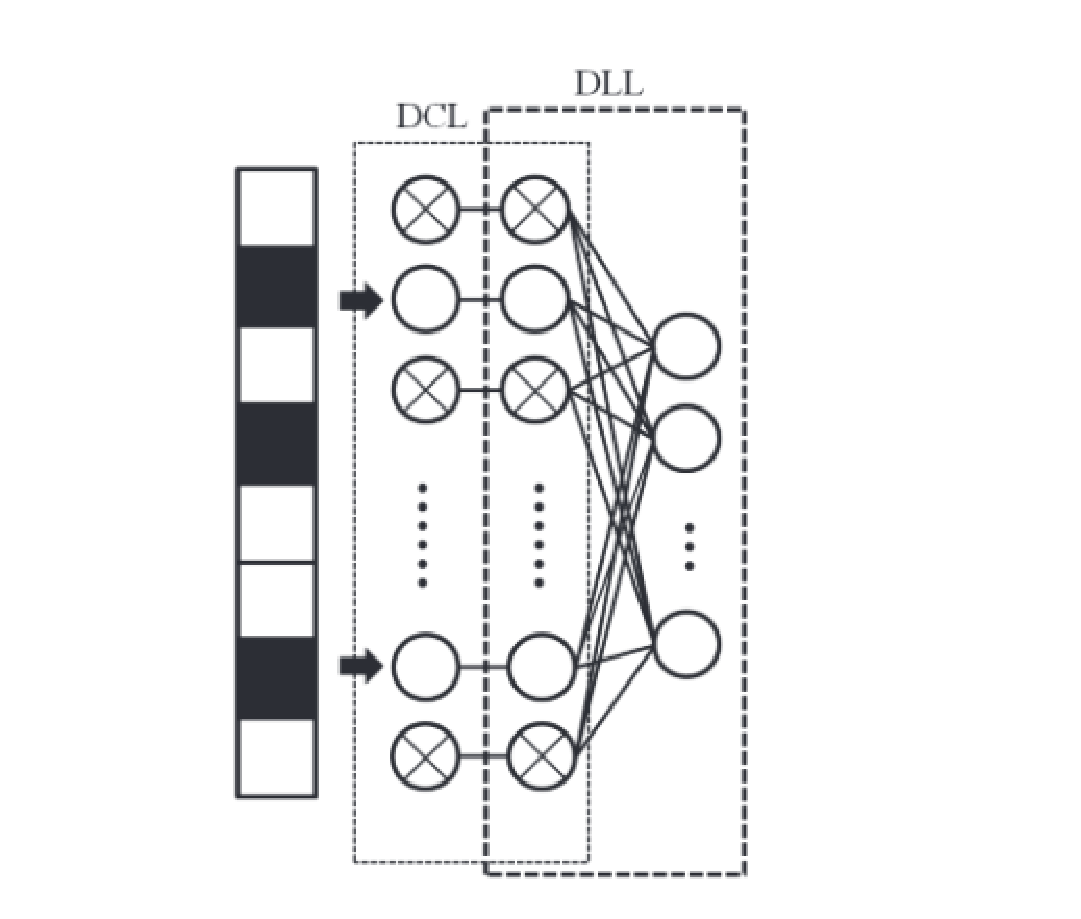
\includegraphics[width=0.6\textwidth]{allpicture/字典学习神经网络结构.eps}
    \caption{字典学习神经网络结构}
    \label{fig:字典学习神经网络结构}
\end{figure}
通过采用分段的训练方法训练稀疏表示的字典,充分学习多样性图像的稀疏表示,
得到了RBM隐藏层神经元的概率分布。神经网络的权值训练采用最优字典矩阵。
测试结果见图~\ref{fig:不同采样率重构图片的PSNR},利用该算法重构的图片的PSNR随着采样率的下降而下降,图片清晰度也显著提高,见图~\ref{fig:重构图像的清晰度对比图}。
\begin{figure}[htpb]
    \centering
    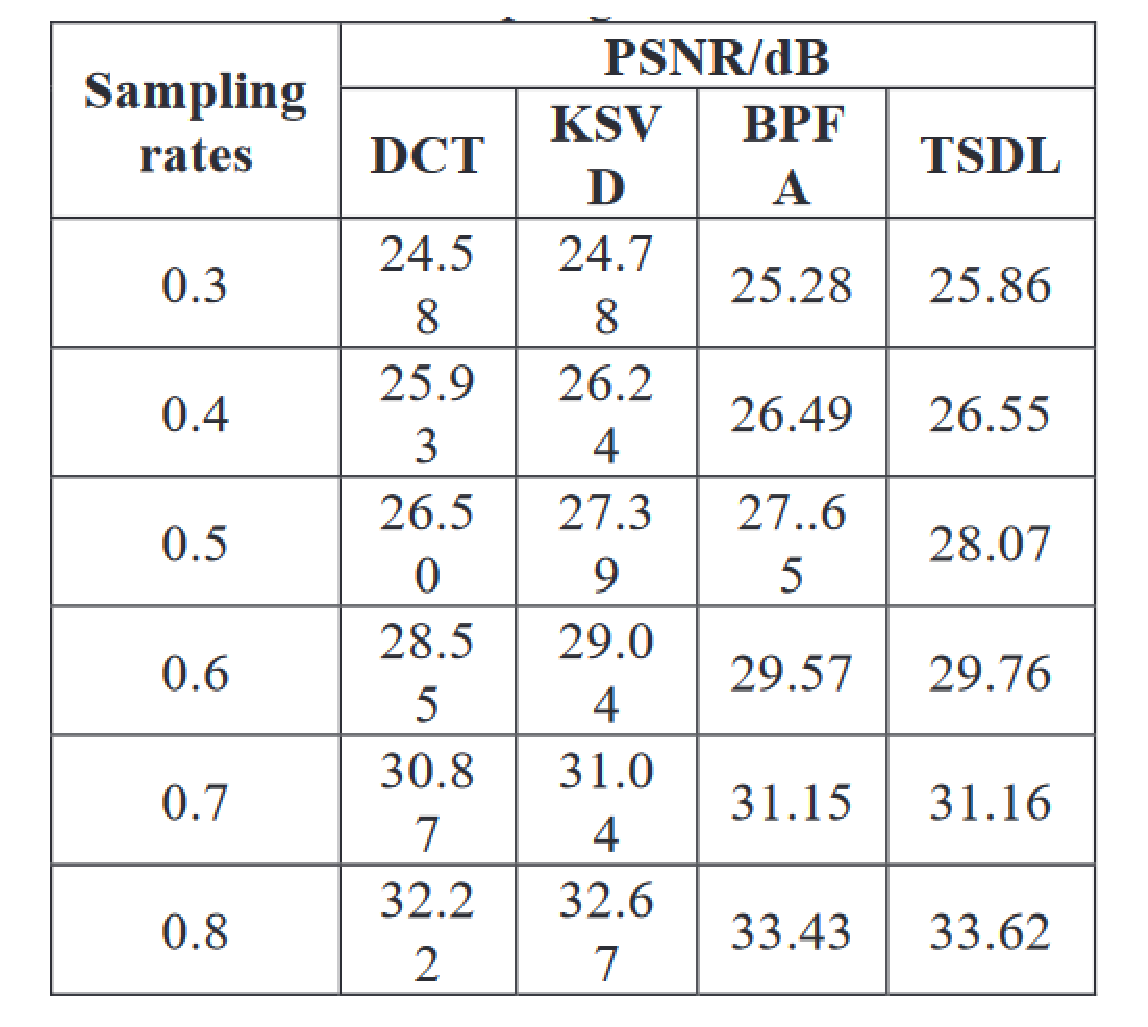
\includegraphics[width=0.6\textwidth]{allpicture/不同采样率重构图片的PSNR.eps}
    \caption{不同采样率重构图片的PSNR}
    \label{fig:不同采样率重构图片的PSNR}
\end{figure}
\begin{figure}[htpb]
    \centering
    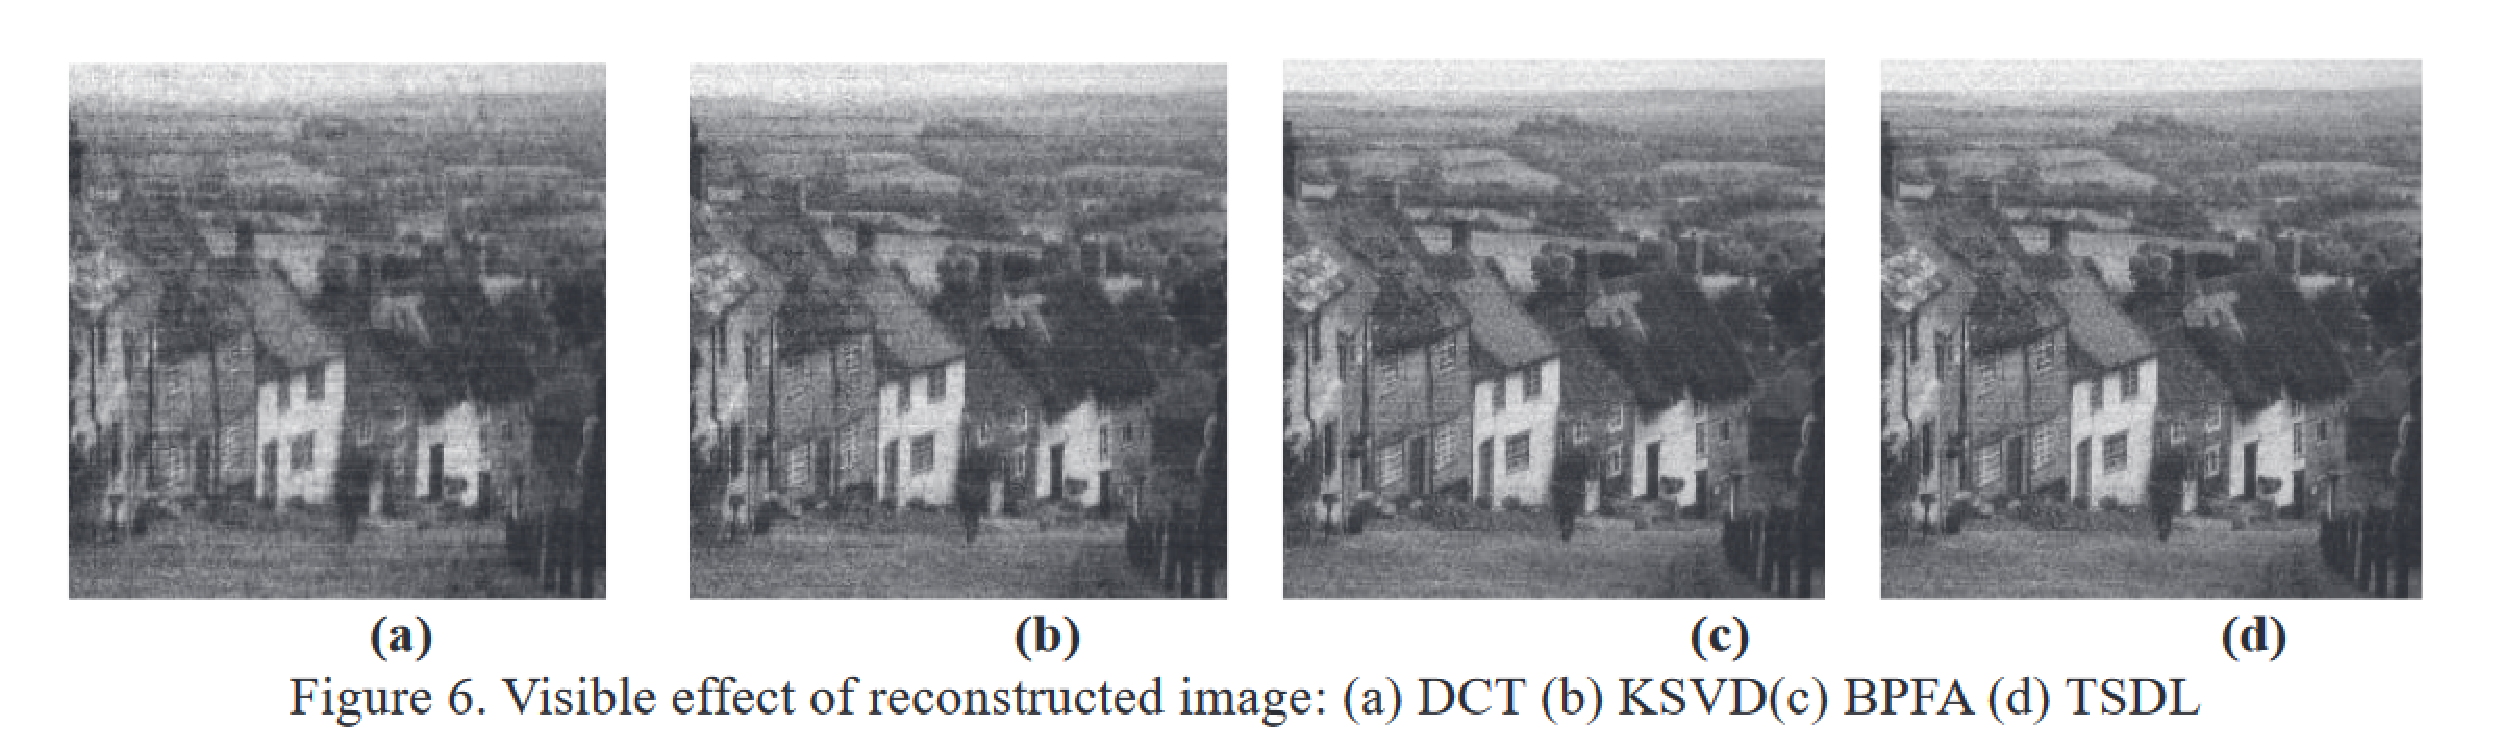
\includegraphics[width=1\textwidth]{allpicture/重构图像的清晰度对比图.eps}
    \caption{重构图像的清晰度对比图}
    \label{fig:重构图像的清晰度对比图}
\end{figure}
实验结果表明,该算法能够提高去噪的效果和提高图片测试的精度。
\section{总结}
本文分为三大块,分别是知识表示与推理、搜索与问题求解以及机器学习的理论和方法。

其中重点内容有:
\begin{itemize}
    \item 确定性推理之启发式搜索算法在危险天气下航班路径规划的应用。
    \item 不确定推理之主观贝叶斯方法在电熔镁炉熔炼过程异常工况识别的应用。
    \item 遗传算法在八皇后问题中的具体实现以及实验设计。
    \item 几种改进的遗传算法在八皇后问题中的具体实现以及实验设计。
    \item 介绍了了人工神经网络的基础架构和常用的几种学习算法。
    \item 介绍了人工神经网络自动编码器算法在信用卡欺诈预警系统的应用。
    \item 介绍了人工神经网络反向传播算法在印尼相关行业股票投资预测方面的应用。
    \item 介绍了基于人工神经网络受限玻尔兹曼机的新型字典学习算法在稀疏图像领域的应用。
\end{itemize}
结论和收获为:
\begin{itemize}
    \item 人工智能是本专业很多研究课题的基础,用心学好这门课可以了解到很多深度学习与机器学习的算法常识。
    \item 从完全不了解人工智能的知识到对基础常用的人工智能算法和模型有了初步的认识。
    \item 从之前只学习过简单直接的经典算法解决问题到现在开始体会到人工智能解决问题的独特方式。
    \item 学习了遗传算法的实现及其使用,以及其在在八皇后问题的具体实现,体会到该算法仿生物学的特性的巧妙。
    \item 学到了文献检索与分类,学习了Zetore文献管理软件的使用,能更快的处理文章编辑过程中的文献插入问题。
    \item 学会了读英文文献的方法流程,磨练了自己的耐心,也非常感谢赵晖老师半年来的授课,我受益匪浅!
\end{itemize}

\bibliographystyle{gbt7714-numerical}
\bibliography{F:/BibTeXref/zoterorepo.bib}
\end{document}